\section{Расчет коэффициента обратной связи, сравнение с результатами Дваера}\label{sec:thunderstorm/rdfm}

Несмотря на то что в хороших условиях в лавине убегающих электронов может быть сгенерировано более миллиона дополнительных электронов, это не объясняет большие потоки гамма-квантов в TGF, а также не дает объяснения как связанны между собой процессы с высокоэнергетичными частицами и разряды молнии. Одним из вариантов модификации теории Гуревича, является построение на её основе модели с обратной связью (ОС). Джозеф Дуайер в работе~\cite{dwyer2003fundamental} предложил рассмотреть два механизма которые могут привести к возникновению обратной связи: гамма обратная связь возникает за счет того что не смотря на то что рождаемые убегающими электронами гамма-квант имеют начальный импульс сонаправленный с направление движения лавины, часть из них в результате рассеяния может в итоге оказаться в части облака в котором начиналась лавина и выбить там электрон, который станет новым затравочным электроном, позитронная обратная связь возникает за счет конверсии гамма-квантов электрон-позитронные пары, при этом позитрон имеет шанс развернутся в электрическом поле и начать ускорятся против направления распространения лавины, выбивая вторичные электроны, которые опять же имеют шанс развернутся в электрическом поле и стать новым затравочным электроном. Рисунок проведенного мною моделирования, иллюстрирует описание позитронной обратной связи: красные треки отображают лавину убегающих электронов, зеленные треки тормозные гамма-кванты, синий трек показывает позитрон обратной связи, который как мы видим создает новые затравочные электроны (которые правда не создают новую лавину). Механизмы описанные Дуайером должны работать в широком диапазоне атмосферных условий, однако являются вероятностными и возникает вопрос насколько значителен вклад этих механизмов в развитие лавин убегающих электронов. В работе~\cite{skeltved2014} повторялись результаты Дуаера, однако без углубленного анализа. В данной работе мы попробуем глубже расмотреть работу этих механизмов.

\begin{figure}[ph!]
    \begin{center}
        \includegraphics[width=\linewidth]{thunderstorm/ayss_2018_art/10_dwyer.pdf}
        \caption{Распространение лавины убегающих электронов, красные треки --- электроны, зеленые треки --- гамма-кванты, синий трек --- позитрон.}
    \end{center}
    \label{fig:storm:dwyer}
\end{figure}

В работе~\cite{dwyer2003fundamental} приводятся результаты моделирования при нормальных условиях исследующие при каких соотношениях длины области с электрическим полем и величины поля может возникать обратная связь. Синяя линия на графике~\ref{fig:storm:dwyer2003} отображает результат полученный Дуаером в ~\cite{dwyer2003fundamental} при значения электрического поля и длины выше этой кривой возникает положительная обратная связь, которая ведёт к значительному росту новых затравочных частиц, который приводит в возникновению TGF и активной ионизации облака достаточной для разряда молнии, в частности подобный результат также говорит что внутри облаков не должно быть скрытых областей с сильным полем --- подобные области должны быстро разряжаться в следствии действия механизмов обратной связи.

Для проверки данных результатов было проведено собственное моделирование, состоящее из двух частей:
\begin{itemize}
	\item Моделирование рождения новых затравочных эелектронов (аналогично работе~\cite{dwyer2003fundamental} электрон считался новым затравочным, если рождался в от гамма-кванта или позитрона в верхней половине облака)за счет гамма и позитронной обратной связи за одну итерацию на одну первичную частицу.
	\item Расчет вероятности с которой электрон может развернутся в электрическом поле. 
\end{itemize}
Для оценки вероятнсти развората было проведено GEANT4 моделирование, для сухого воздуха при нормальных условиях, величины электрического поля бралась от 5 до 10 кВ/см с шагом 0.5 кВ/см. Результат расчета вероятности разворота представлена на рисунках~\ref{fig:storm:reverse_nc_1} и ~\ref{fig:storm:reverse_nc_2}. Так же что бы быть увереным что электрон после разворота сможет начать движение была расчитанна средняя энергия элеткрона после разворота, результаты приведены на графиках~\ref{fig:storm:reverse_energy_nc_1} и ~\ref{fig:storm:reverse_energy_nc_2}, как видно из графиков хоть электрон и тратит энергию на разворот, она остатется достаточной для запуска новой лавины убегающих электронов (см. график TODO(график), показывающий минимальную энергию для начала убегания).  

\begin{figure}[ph!]
    \begin{center}
        \begin{minipage}[h]{0.49\linewidth}
            \center{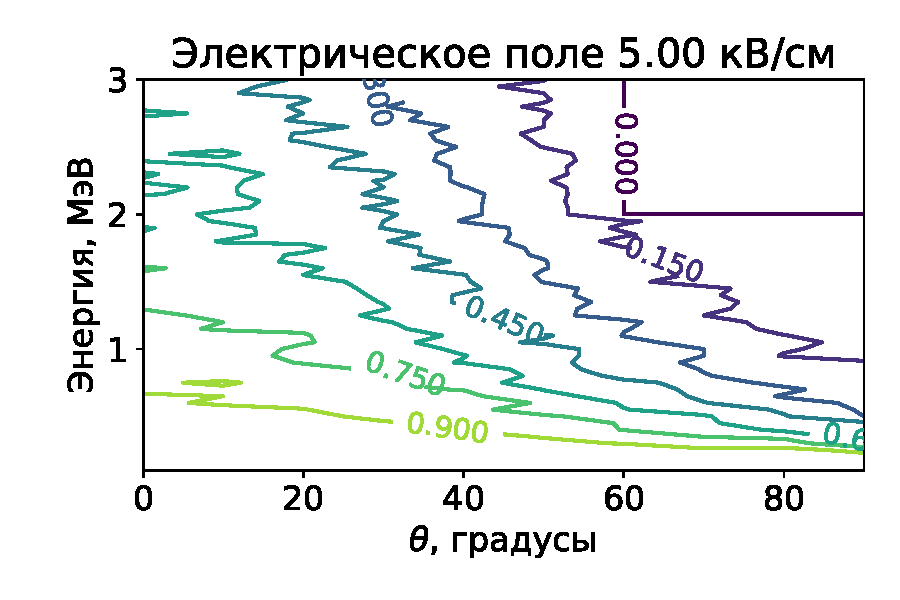
\includegraphics[width=\linewidth]{thunderstorm/rdfm/reverse_5_00.pdf} \\ а)}
        \end{minipage}
        \hfill
        \begin{minipage}[h]{0.49\linewidth}
            \center{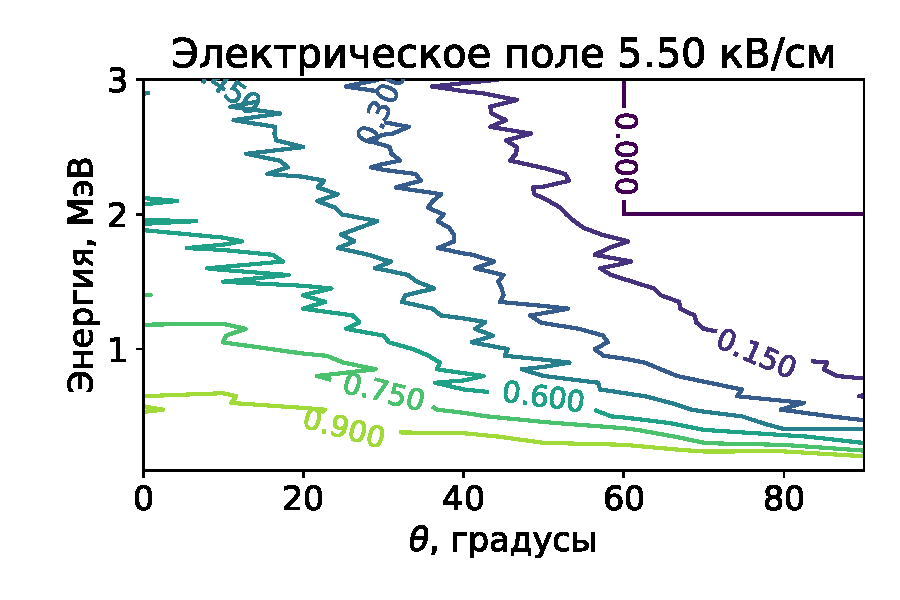
\includegraphics[width=\linewidth]{thunderstorm/rdfm/reverse_5_50.pdf} \\ б)}
        \end{minipage}
        \vfill
        \begin{minipage}[h]{0.49\linewidth}
            \center{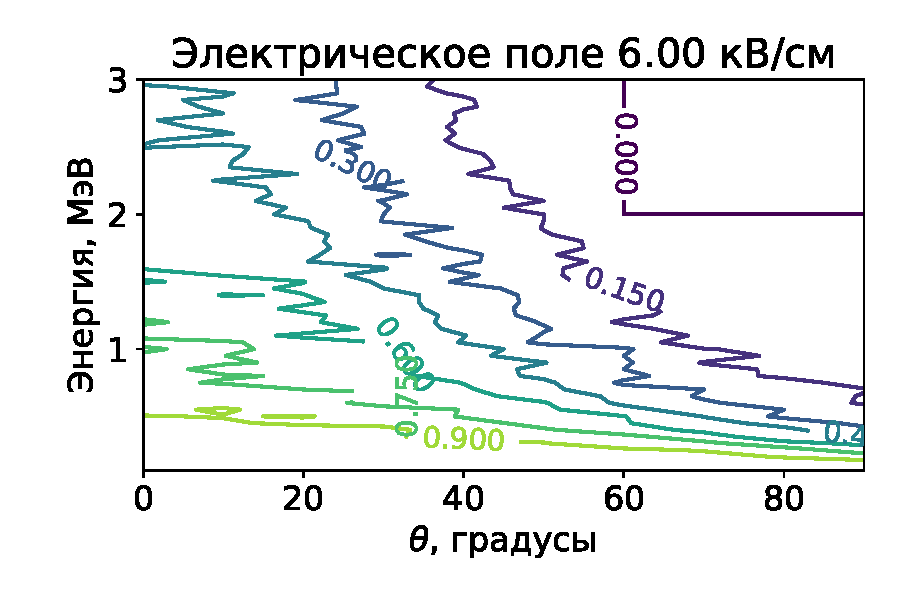
\includegraphics[width=\linewidth]{thunderstorm/rdfm/reverse_6_00.pdf} \\ в)}
        \end{minipage}
        \hfill
        \begin{minipage}[h]{0.49\linewidth}
            \center{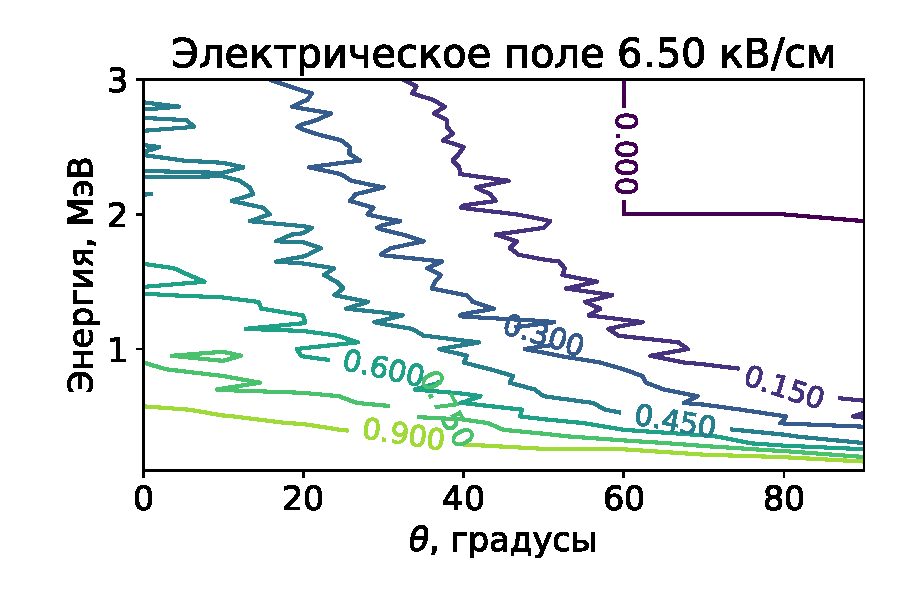
\includegraphics[width=\linewidth]{thunderstorm/rdfm/reverse_6_50.pdf} \\ г)}
        \end{minipage}
        \vfill
        \begin{minipage}[h]{0.49\linewidth}
            \center{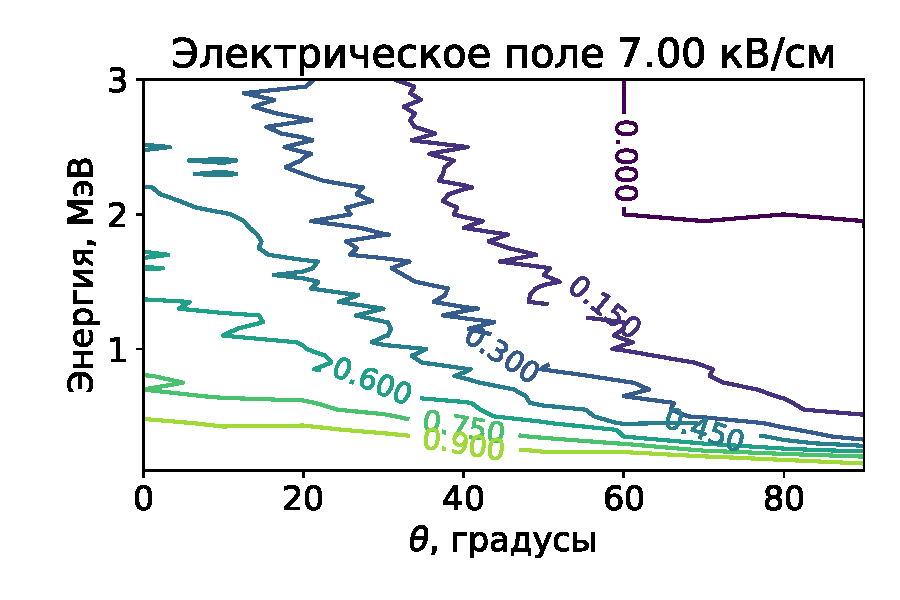
\includegraphics[width=\linewidth]{thunderstorm/rdfm/reverse_7_00.pdf} \\ д)}
        \end{minipage}
        \hfill
        \begin{minipage}[h]{0.49\linewidth}
            \center{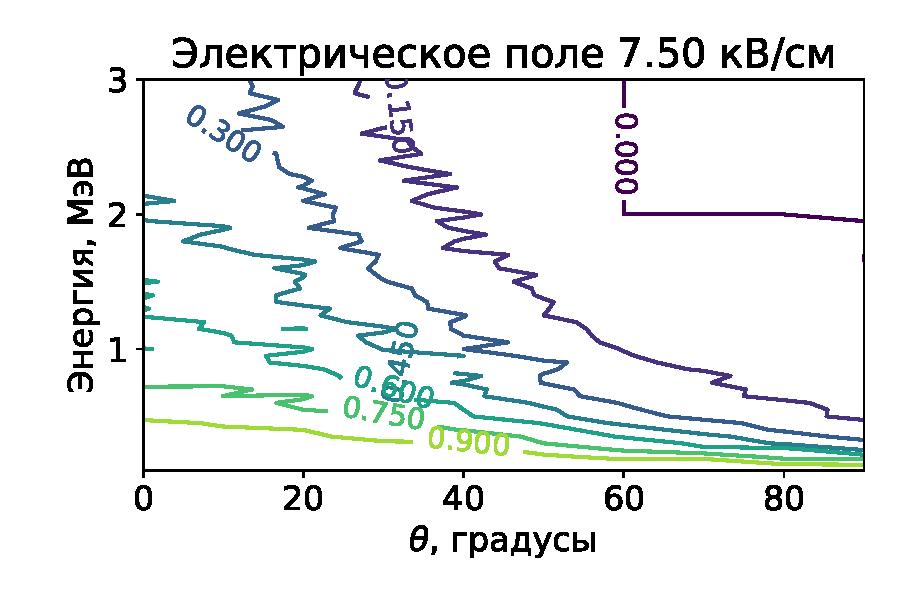
\includegraphics[width=\linewidth]{thunderstorm/rdfm/reverse_7_50.pdf} \\ е)}
        \end{minipage}
        \caption{Расчет вероятности электрона равзернутся в электрическом поле для нормальных условий. По оси X отображается угол между направление движения TODO(перерисовать угол на графике), а по оси Y энергия электроно. На графики отображены линии с постоянной вероятность разворота и числовое знаение вероятности на линии.}
    \end{center}
    \label{fig:storm:reverse_nc_1}
\end{figure}
\begin{figure}[ph!]
    \begin{center}
        \begin{minipage}[h]{0.49\linewidth}
            \center{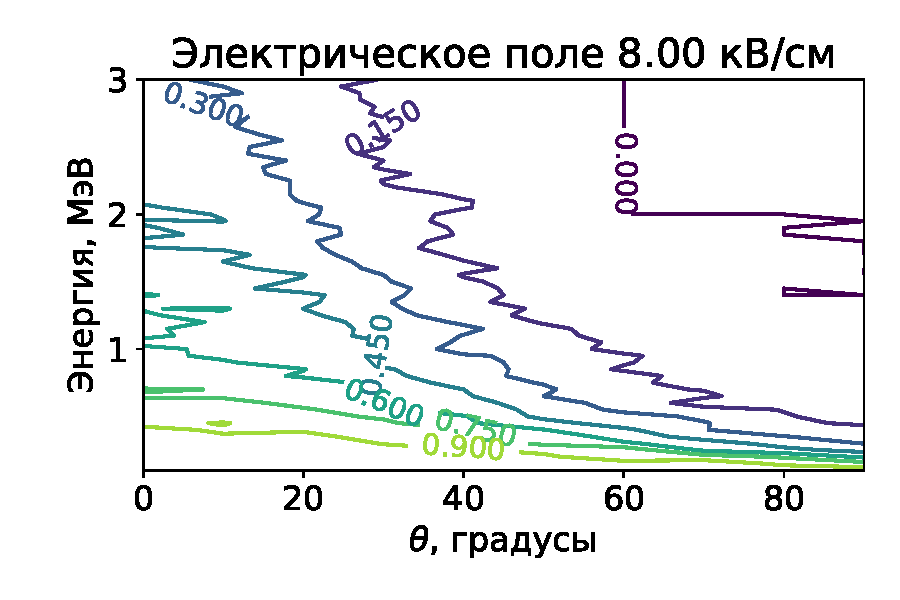
\includegraphics[width=\linewidth]{thunderstorm/rdfm/reverse_8_00.pdf} \\ ж)}
        \end{minipage}
        \hfill
        \begin{minipage}[h]{0.49\linewidth}
            \center{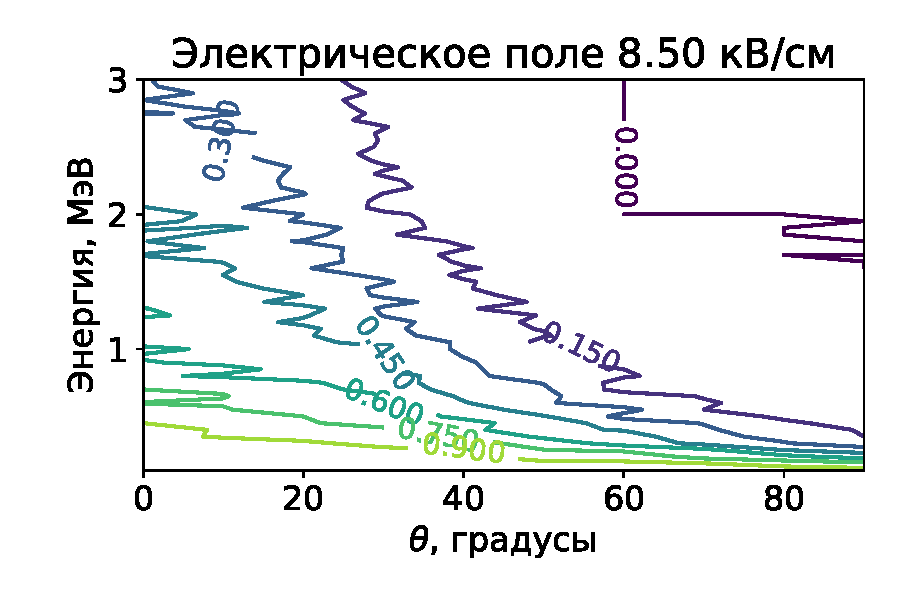
\includegraphics[width=\linewidth]{thunderstorm/rdfm/reverse_8_50.pdf} \\ з)}
        \end{minipage}    
        \vfill
        \begin{minipage}[h]{0.49\linewidth}
            \center{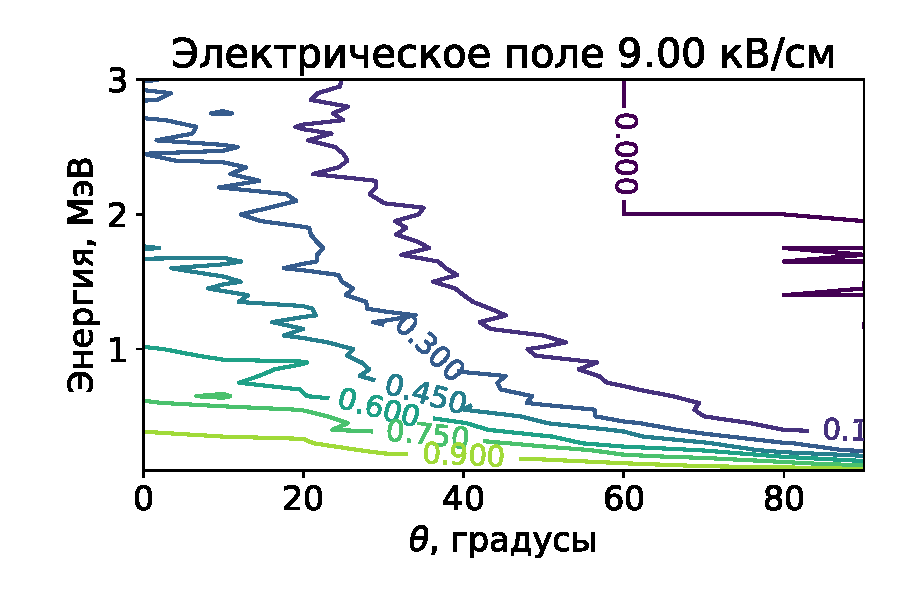
\includegraphics[width=\linewidth]{thunderstorm/rdfm/reverse_9_00.pdf} \\ и)}
        \end{minipage}
        \hfill
        \begin{minipage}[h]{0.49\linewidth}
            \center{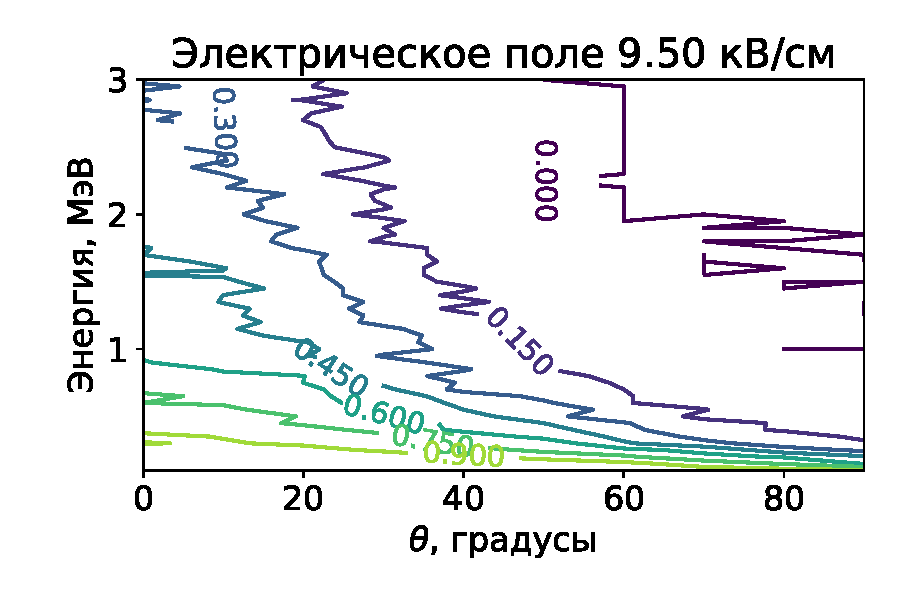
\includegraphics[width=\linewidth]{thunderstorm/rdfm/reverse_9_50.pdf} \\ к)}
        \end{minipage} 
        \vfill
        \begin{minipage}[h]{0.49\linewidth}
            \center{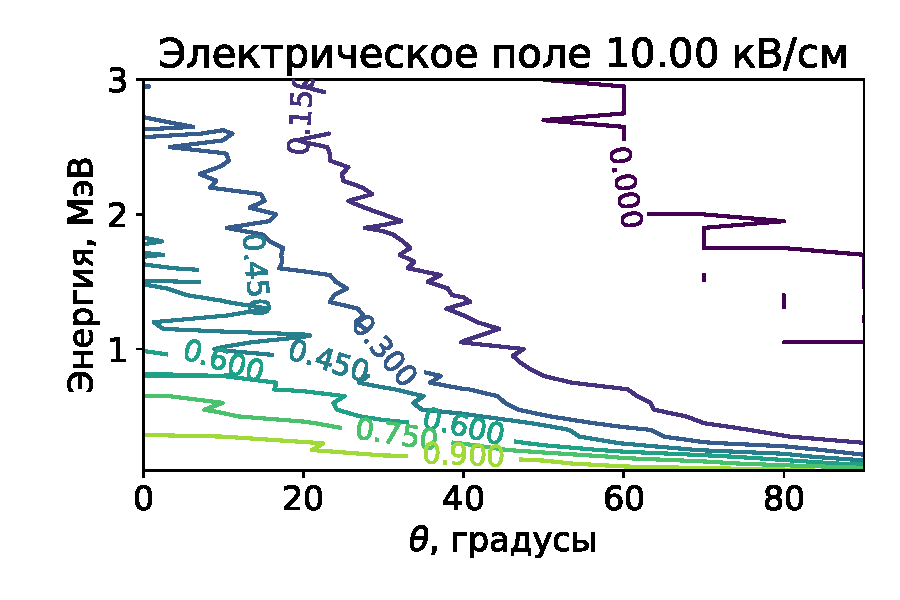
\includegraphics[width=\linewidth]{thunderstorm/rdfm/reverse_10_00.pdf} \\ л)}
        \end{minipage}
        \caption{Разворот электрона TODO(Скопировать)}
    \end{center}
    \label{fig:storm:reverse_nc_2}
\end{figure}


\begin{figure}[ph!]
    \begin{center}
        \begin{minipage}[h]{0.49\linewidth}
            \center{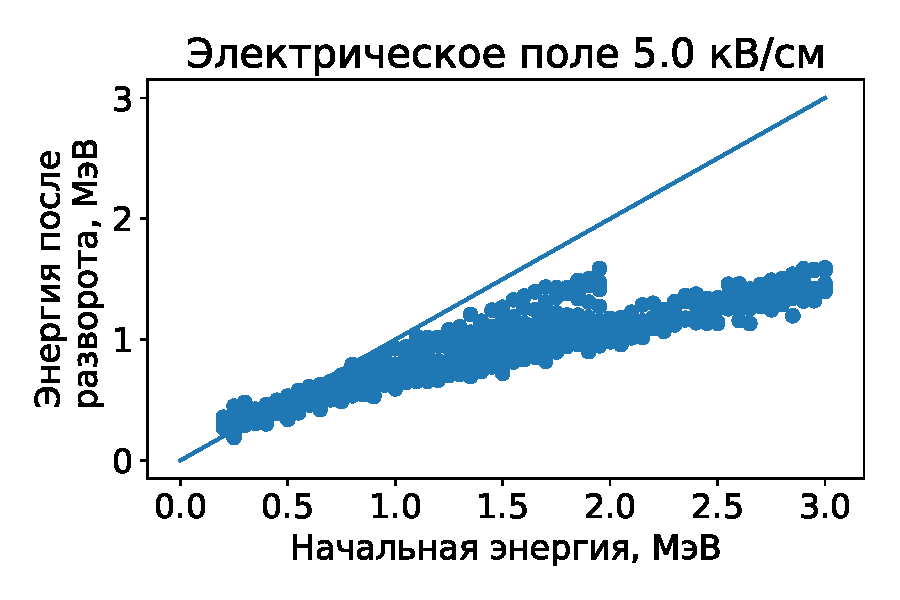
\includegraphics[width=\linewidth]{thunderstorm/rdfm/reverse_energy_5_0.pdf} \\ а)}
        \end{minipage}
        \hfill
        \begin{minipage}[h]{0.49\linewidth}
            \center{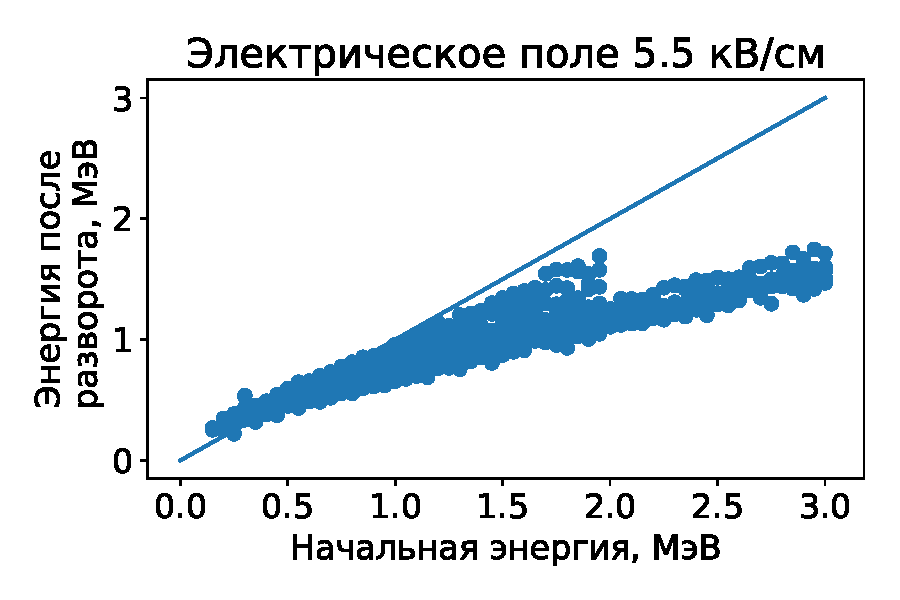
\includegraphics[width=\linewidth]{thunderstorm/rdfm/reverse_energy_5_5.pdf} \\ б)}
        \end{minipage}
        \vfill
        \begin{minipage}[h]{0.49\linewidth}
            \center{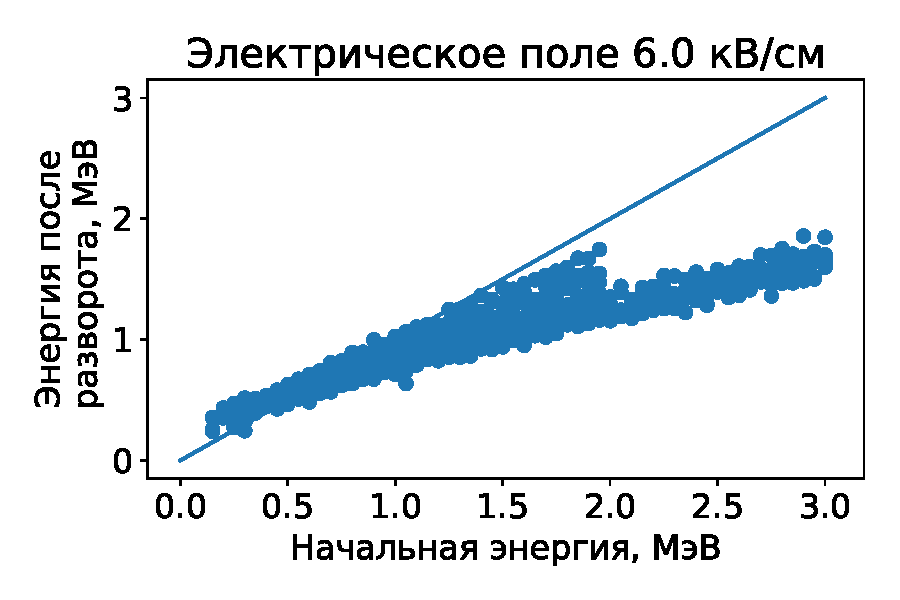
\includegraphics[width=\linewidth]{thunderstorm/rdfm/reverse_energy_6_0.pdf} \\ в)}
        \end{minipage}
        \hfill
        \begin{minipage}[h]{0.49\linewidth}
            \center{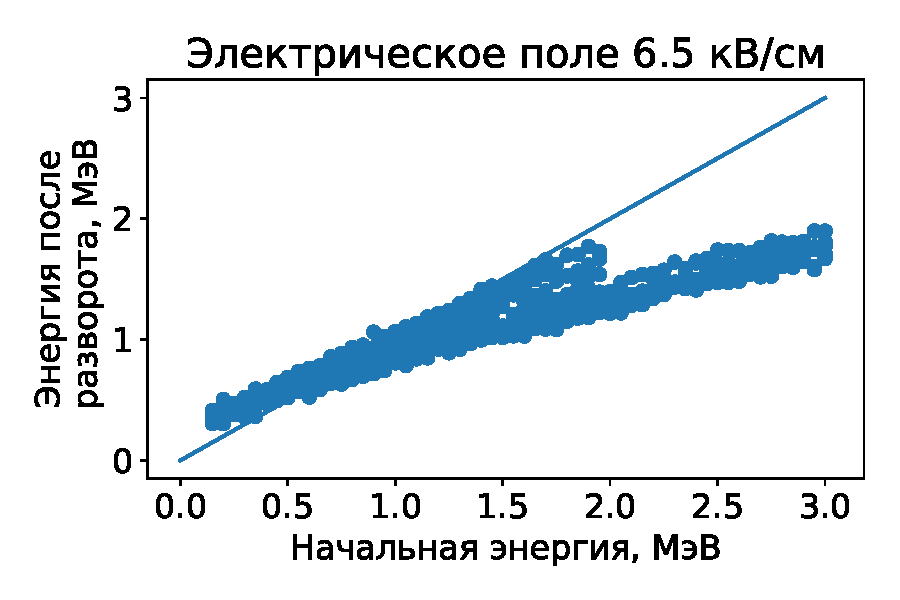
\includegraphics[width=\linewidth]{thunderstorm/rdfm/reverse_energy_6_5.pdf} \\ г)}
        \end{minipage}
        \vfill
        \begin{minipage}[h]{0.49\linewidth}
            \center{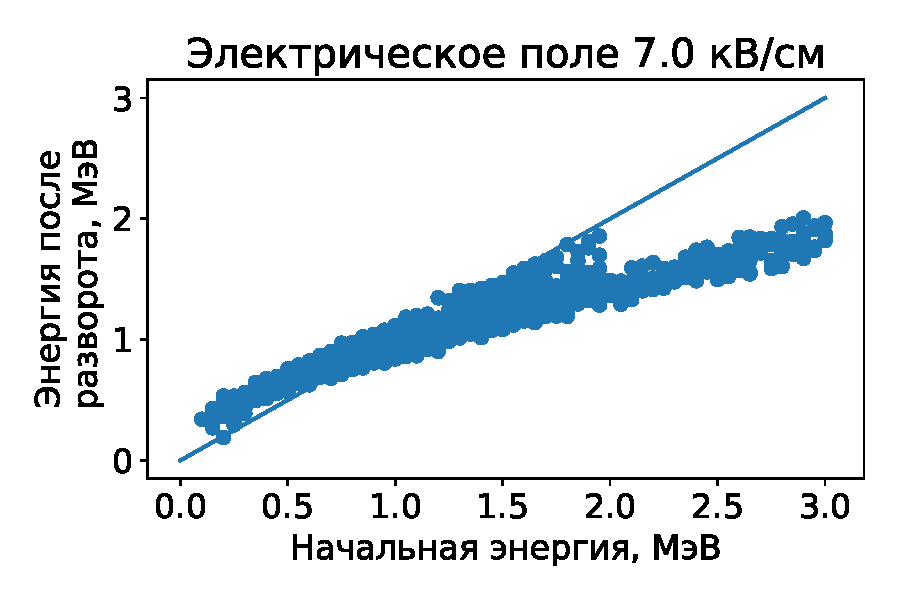
\includegraphics[width=\linewidth]{thunderstorm/rdfm/reverse_energy_7_0.pdf} \\ д)}
        \end{minipage}
        \hfill
        \begin{minipage}[h]{0.49\linewidth}
            \center{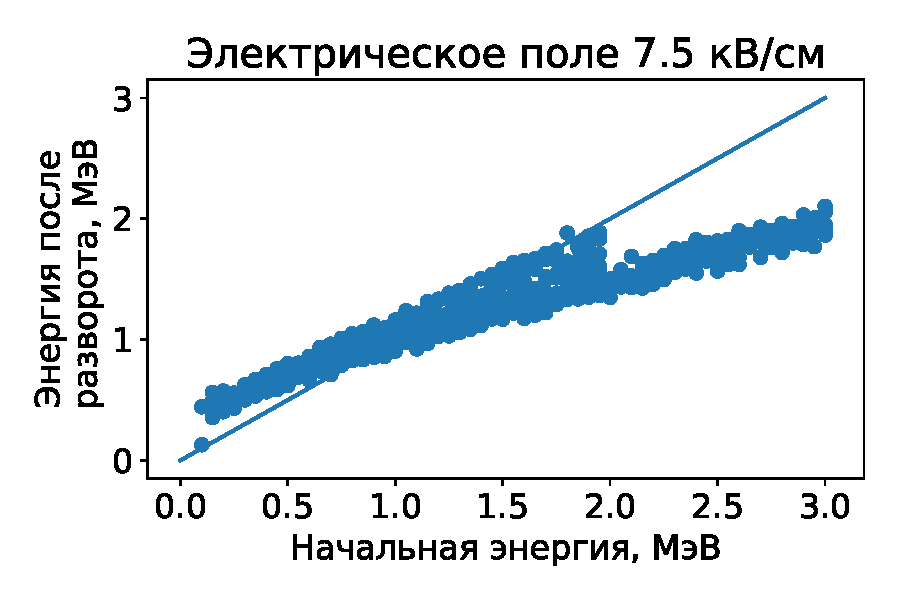
\includegraphics[width=\linewidth]{thunderstorm/rdfm/reverse_energy_7_5.pdf} \\ е)}
        \end{minipage}
        \caption{Зависимость средней энергии электрона после разворота от начальной энергии для разных значений электрического поля.}
    \end{center}
    \label{fig:storm:reverse_energy_nc_1}
\end{figure}
\begin{figure}[ph!]
    \begin{center}
        \begin{minipage}[h]{0.49\linewidth}
            \center{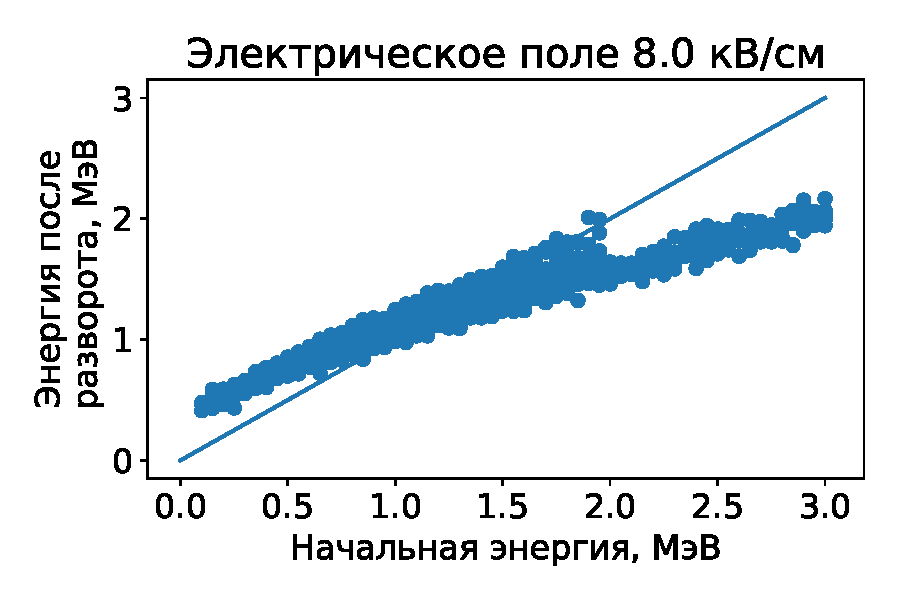
\includegraphics[width=\linewidth]{thunderstorm/rdfm/reverse_energy_8_0.pdf} \\ ж)}
        \end{minipage}
        \hfill
        \begin{minipage}[h]{0.49\linewidth}
            \center{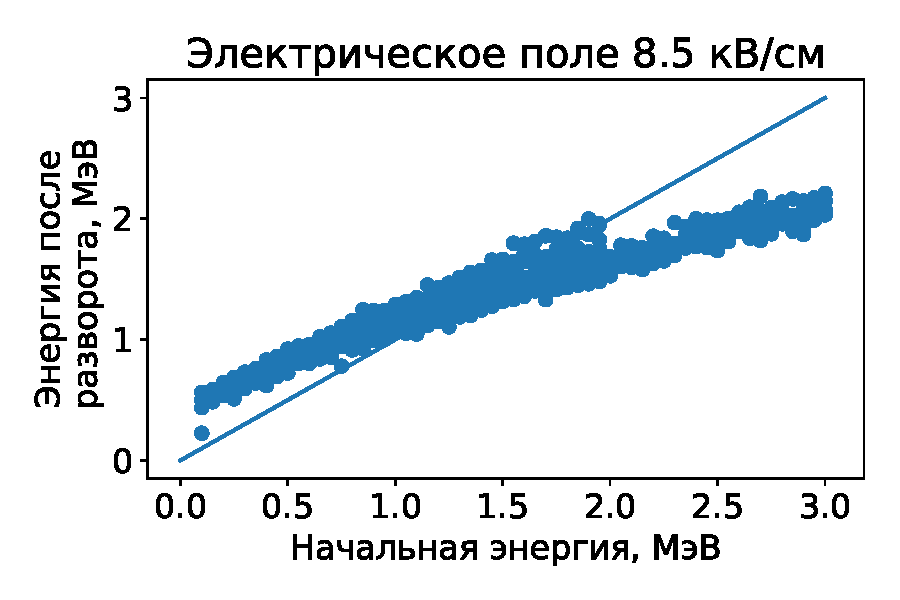
\includegraphics[width=\linewidth]{thunderstorm/rdfm/reverse_energy_8_5.pdf} \\ з)}
        \end{minipage}    
        \vfill
        \begin{minipage}[h]{0.49\linewidth}
            \center{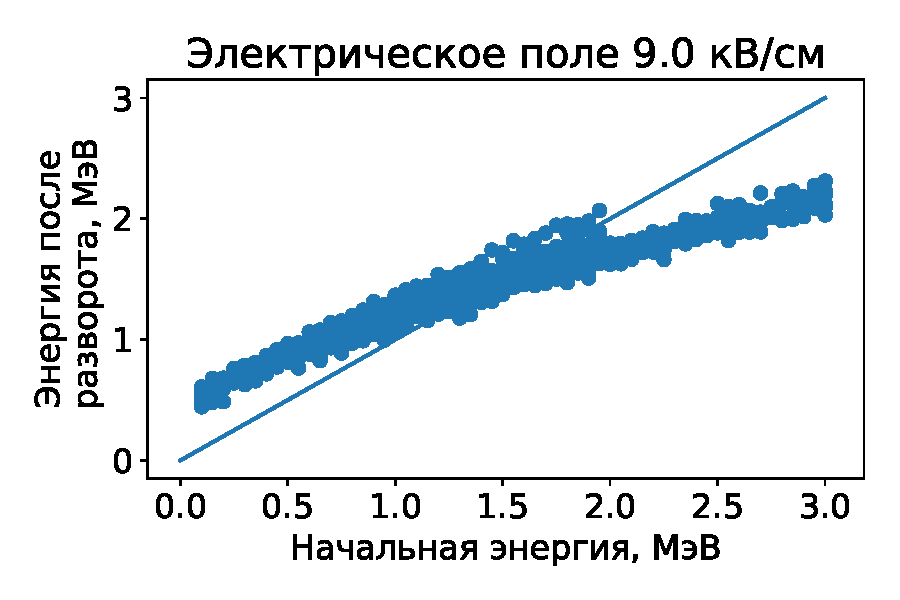
\includegraphics[width=\linewidth]{thunderstorm/rdfm/reverse_energy_9_0.pdf} \\ и)}
        \end{minipage}
        \hfill
        \begin{minipage}[h]{0.49\linewidth}
            \center{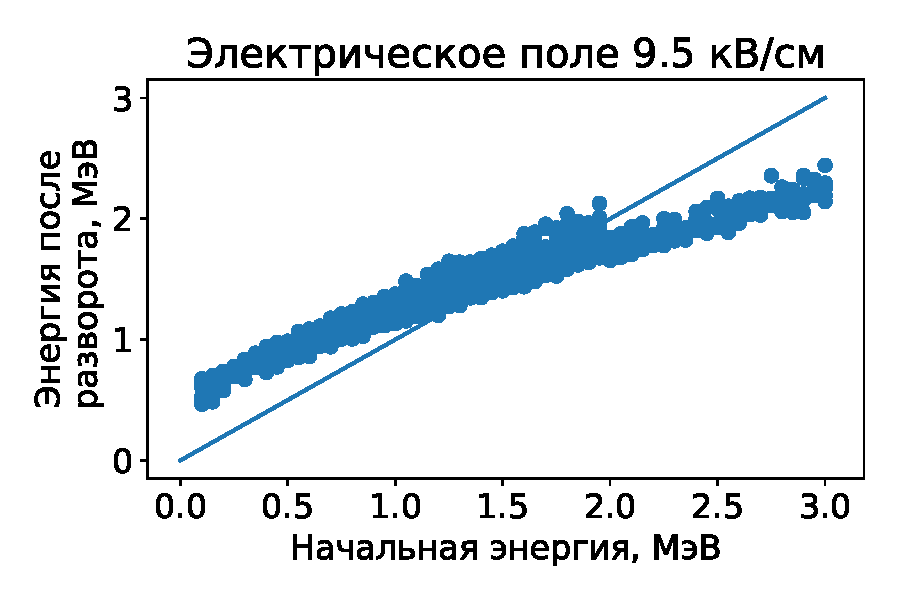
\includegraphics[width=\linewidth]{thunderstorm/rdfm/reverse_energy_9_5.pdf} \\ к)}
        \end{minipage} 
        \vfill
        \begin{minipage}[h]{0.49\linewidth}
            \center{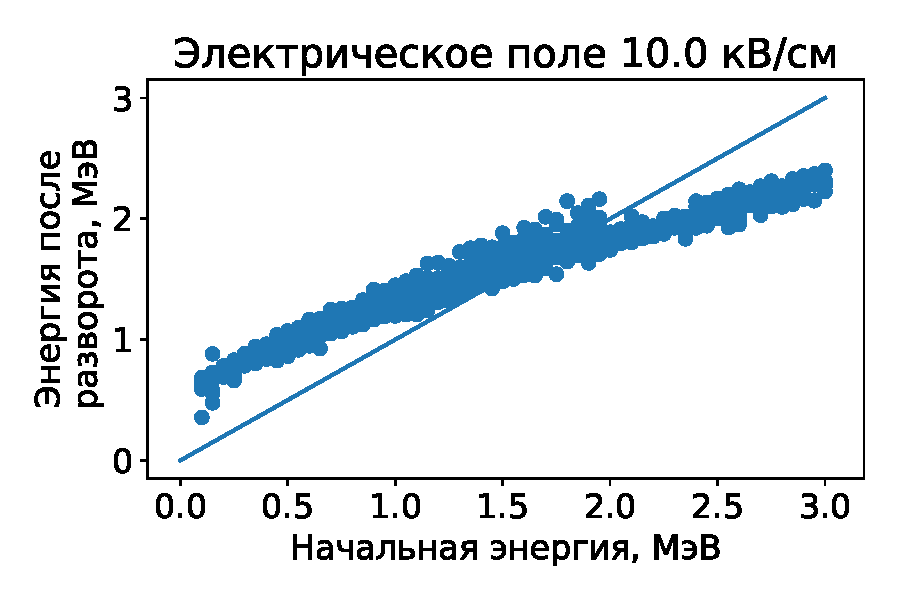
\includegraphics[width=\linewidth]{thunderstorm/rdfm/reverse_energy_10_0.pdf} \\ л)}
        \end{minipage}
        \caption{Зависимость средней энергии электрона после разворота от начальной энергии для разных значений электрического поля.}
    \end{center}
    \label{fig:storm:reverse_energy_nc_2}
\end{figure}
Далее было провдено моделирование рождения новых затравчных электронов, для этого было взято несколько точек вдоль и чуть выше кривой полученной Дуаером (отмечены на графике~\ref{fig:storm:dwyer2003}а красными трегольниками), и для данных точек было сделано GEANT4 моделирование лавины убегающих электронов.  Для каждой точки было рассчитано число новых затравочных электронов рожденных с помощью позитронов и гамма-квантов с учетом вероятности развернутся в электрическом поле, результаты представлены в таблице~\ref{tab:storm:dwyer}. Из провденного моделирования можно сделать следующие выводы:
\begin{itemize}
	\item Результаты моделирования согласуются с результатими Дуаера, однако в отличии от него мы получили не просто качетсвенную оценку наличия/отсутвия новых затравочных частиц, но и получили количетсвенные оценки, также далее мы проведем структурны анализ новых затравочных электронов и покажем некоторые проблемы которые могут значительно уменьшать эффективность работы механизмов обратной связи.
	\item Наша количетсванная оценка позволяет сдеать интресное наблюдение: на эфффективность работы механизмов обратной связи в большей стпени влияет длинна обалсти с полем, чем величина поля. Это важный результат так как он говорит о проблемах стримерной гипотезы возникновения TGF, подробнее см раздел TODO(Раздел). 
\end{itemize}

\begin{figure}[t]
    \begin{center}
        \begin{minipage}[h]{0.49\linewidth}
            \center{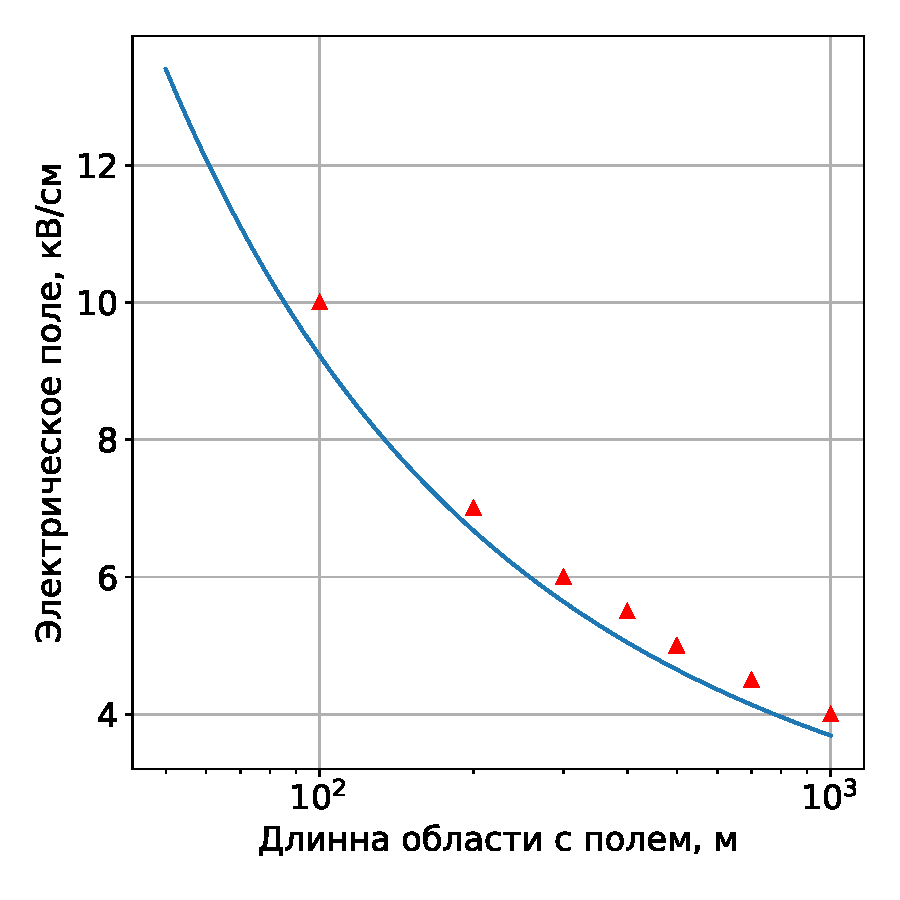
\includegraphics[width=\linewidth]{thunderstorm/rdfm/dwyer_2003.pdf} \\ а)}
        \end{minipage}
        \hfill
        \begin{minipage}[h]{0.49\linewidth}
            \center{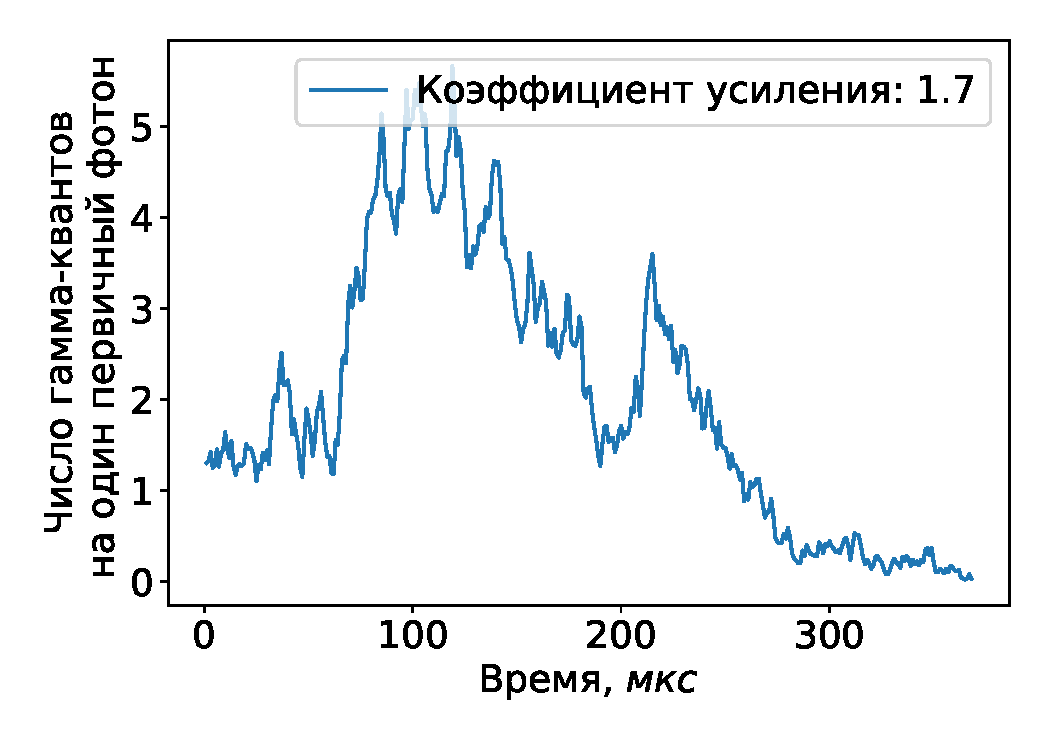
\includegraphics[width=\linewidth]{thunderstorm/RL_Extinction.pdf}   \\ б)}
        \end{minipage}
        \caption{а) Затухание лавины. б) placeholder.}
    \end{center}
    \label{fig:storm:dwyer2003}
\end{figure}

\begin{table}[h]
    \centering
    \begin{tabular}{crrrr}
        \hline
        & & & \multicolumn{2}{r}{Число новых затравочных электронов} \\
        & Поле, кВ/см &  Длина облака, м  & от гамма ОС & от позитронной ОС \\
        \hline
        & 4   &  1000&  0 & 0  \\
        & 4.5 &  700 &  200 ($\pm 10 \%$)& 400 ($\pm 5 \%$) \\
        & 5   &  500 &  100 ($\pm 14 \%$)& 40 ($\pm 5 \%$) \\
        & 5.5 &  400 &  110 ($\pm 3 \%$)& 85 ($\pm 5 \%$) \\
        & 6   &  300 &  40 ($\pm 3 \%$)& 70 ($\pm 2 \%$) \\
        & 7   &  200 &  7 ($\pm 2 \%$)& 8 ($\pm 2 \%$) \\
        & 10  &  100 &  5 ($\pm 3 \%$)& 2 ($\pm 5 \%$) \\
        \hline
    \end{tabular}
    \caption{Моделирование числа новых затравочных электронов возникающих за счет одной итерации механизма обратной связи на один первичный электрон.}
    \label{tab:storm:dwyer}
\end{table}

Однако не смотря на то что наши результат совпали с результатами Дуаера, у его модели обратной связи можно отмеить несколько недостатков. 

Моделирование Дуайера проводилось при нормальных условиях, то есть для атмосферы лежащей на уровне моря, однако реальные явления происходят больших высотах (например, на научных станциях на г. Арагац и на Тянь Шане производится наблюдене за грозовыми облаками идущими на высотах 3-5 километра, а спутниковые наблдюдения говрят об источниках TGF расположенных на высотах 12-15 киометров). Можно провести экстрополяцию от нормалных условий к условиям на больших высотах, считатая что величины (такие как критическое  поле или поле для возникновения обратной связи) уменьшаются пропорционально плотности, а растояния увеичиваются пропорционално плотности, как было предложен Дуаером, однако такие предположения имеет ограниченную точность. Например, проведенный в разделе ~\ref{sec:thunderstorm/rrea} расчет характерной длинны нарастания лавины был проведен при условиях соответвующей 10 километровой высоте и сравнивался с величиной полученной Дуаером, которая была расчитана при нормальных условиях и экстраполирована к условия высота 10 км, полученные результат отличаются, хоть они и не дают такого различия как результаты полученные в работе~\cite{oreshkin2018}, но в рамках сравнения наших моделирований отличие сущетсвенно и может свидетельствоать он не правомерноси интреполяции результатов полученных при норальных условиях к условиях на больших высотах. 

Другим недостатком расчетов Дуаера является пренебрежение реальными размерами облака, для пример расматрим радиальное распределение образования убегающих электронов показаное на рис.~\ref{fig:storm:dwyer2003} TODO(рисунок). Видно, что электроны имеют широкое горизонтальное распределение которе может сравнимым с размером небольшого облака. Дополнтельно следует учесть что фотоны могут переносить вторичные лавины далеко от начальных, или активно покидать облако, рисунок TODO(рисунок радиального распредления затравоных частиц)

Так важно учесть нетолько распределение в горизонтальном простантсве, но и по вертикали. Обычно в моделирвании мы размещаем затравочнуя частицу в начале области с электрическим полем, однако новые затравочные частицы родаемые за счет гамма или позитронной обратной связи имееют некоторое распредление по вертикали (см. рис)





